\PassOptionsToPackage{unicode=true}{hyperref} % options for packages loaded elsewhere
\PassOptionsToPackage{hyphens}{url}
%
\documentclass[]{krantz}
\usepackage{lmodern}
\usepackage{amssymb,amsmath}
\usepackage{ifxetex,ifluatex}
\usepackage{fixltx2e} % provides \textsubscript
\ifnum 0\ifxetex 1\fi\ifluatex 1\fi=0 % if pdftex
  \usepackage[T1]{fontenc}
  \usepackage[utf8]{inputenc}
  \usepackage{textcomp} % provides euro and other symbols
\else % if luatex or xelatex
  \usepackage{unicode-math}
  \defaultfontfeatures{Ligatures=TeX,Scale=MatchLowercase}
\fi
% use upquote if available, for straight quotes in verbatim environments
\IfFileExists{upquote.sty}{\usepackage{upquote}}{}
% use microtype if available
\IfFileExists{microtype.sty}{%
\usepackage[]{microtype}
\UseMicrotypeSet[protrusion]{basicmath} % disable protrusion for tt fonts
}{}
\IfFileExists{parskip.sty}{%
\usepackage{parskip}
}{% else
\setlength{\parindent}{0pt}
\setlength{\parskip}{6pt plus 2pt minus 1pt}
}
\usepackage{hyperref}
\hypersetup{
            pdftitle={Un libro},
            pdfauthor={Ricardo Michel MALLQUI BAÑOS},
            pdfborder={0 0 0},
            breaklinks=true}
\urlstyle{same}  % don't use monospace font for urls
\usepackage{color}
\usepackage{fancyvrb}
\newcommand{\VerbBar}{|}
\newcommand{\VERB}{\Verb[commandchars=\\\{\}]}
\DefineVerbatimEnvironment{Highlighting}{Verbatim}{commandchars=\\\{\}}
% Add ',fontsize=\small' for more characters per line
\usepackage{framed}
\definecolor{shadecolor}{RGB}{248,248,248}
\newenvironment{Shaded}{\begin{snugshade}}{\end{snugshade}}
\newcommand{\AlertTok}[1]{\textcolor[rgb]{0.33,0.33,0.33}{#1}}
\newcommand{\AnnotationTok}[1]{\textcolor[rgb]{0.37,0.37,0.37}{\textbf{\textit{#1}}}}
\newcommand{\AttributeTok}[1]{\textcolor[rgb]{0.61,0.61,0.61}{#1}}
\newcommand{\BaseNTok}[1]{\textcolor[rgb]{0.06,0.06,0.06}{#1}}
\newcommand{\BuiltInTok}[1]{#1}
\newcommand{\CharTok}[1]{\textcolor[rgb]{0.5,0.5,0.5}{#1}}
\newcommand{\CommentTok}[1]{\textcolor[rgb]{0.37,0.37,0.37}{\textit{#1}}}
\newcommand{\CommentVarTok}[1]{\textcolor[rgb]{0.37,0.37,0.37}{\textbf{\textit{#1}}}}
\newcommand{\ConstantTok}[1]{\textcolor[rgb]{0,0,0}{#1}}
\newcommand{\ControlFlowTok}[1]{\textcolor[rgb]{0.27,0.27,0.27}{\textbf{#1}}}
\newcommand{\DataTypeTok}[1]{\textcolor[rgb]{0.27,0.27,0.27}{#1}}
\newcommand{\DecValTok}[1]{\textcolor[rgb]{0.06,0.06,0.06}{#1}}
\newcommand{\DocumentationTok}[1]{\textcolor[rgb]{0.37,0.37,0.37}{\textbf{\textit{#1}}}}
\newcommand{\ErrorTok}[1]{\textcolor[rgb]{0.14,0.14,0.14}{\textbf{#1}}}
\newcommand{\ExtensionTok}[1]{#1}
\newcommand{\FloatTok}[1]{\textcolor[rgb]{0.06,0.06,0.06}{#1}}
\newcommand{\FunctionTok}[1]{\textcolor[rgb]{0,0,0}{#1}}
\newcommand{\ImportTok}[1]{#1}
\newcommand{\InformationTok}[1]{\textcolor[rgb]{0.37,0.37,0.37}{\textbf{\textit{#1}}}}
\newcommand{\KeywordTok}[1]{\textcolor[rgb]{0.27,0.27,0.27}{\textbf{#1}}}
\newcommand{\NormalTok}[1]{#1}
\newcommand{\OperatorTok}[1]{\textcolor[rgb]{0.43,0.43,0.43}{\textbf{#1}}}
\newcommand{\OtherTok}[1]{\textcolor[rgb]{0.37,0.37,0.37}{#1}}
\newcommand{\PreprocessorTok}[1]{\textcolor[rgb]{0.37,0.37,0.37}{\textit{#1}}}
\newcommand{\RegionMarkerTok}[1]{#1}
\newcommand{\SpecialCharTok}[1]{\textcolor[rgb]{0,0,0}{#1}}
\newcommand{\SpecialStringTok}[1]{\textcolor[rgb]{0.5,0.5,0.5}{#1}}
\newcommand{\StringTok}[1]{\textcolor[rgb]{0.5,0.5,0.5}{#1}}
\newcommand{\VariableTok}[1]{\textcolor[rgb]{0,0,0}{#1}}
\newcommand{\VerbatimStringTok}[1]{\textcolor[rgb]{0.5,0.5,0.5}{#1}}
\newcommand{\WarningTok}[1]{\textcolor[rgb]{0.37,0.37,0.37}{\textbf{\textit{#1}}}}
\usepackage{longtable,booktabs}
% Fix footnotes in tables (requires footnote package)
\IfFileExists{footnote.sty}{\usepackage{footnote}\makesavenoteenv{longtable}}{}
\setlength{\emergencystretch}{3em}  % prevent overfull lines
\providecommand{\tightlist}{%
  \setlength{\itemsep}{0pt}\setlength{\parskip}{0pt}}
\setcounter{secnumdepth}{5}
% Redefines (sub)paragraphs to behave more like sections
\ifx\paragraph\undefined\else
\let\oldparagraph\paragraph
\renewcommand{\paragraph}[1]{\oldparagraph{#1}\mbox{}}
\fi
\ifx\subparagraph\undefined\else
\let\oldsubparagraph\subparagraph
\renewcommand{\subparagraph}[1]{\oldsubparagraph{#1}\mbox{}}
\fi

% set default figure placement to htbp
\makeatletter
\def\fps@figure{htbp}
\makeatother

\usepackage[spanish,english]{babel}
\usepackage{booktabs}
\usepackage{graphicx}
\usepackage{makeidx}
\makeindex
\usepackage{imakeidx}
%\usepackage{showframe}
\makeindex[columns=2, title=\'Indice ]

\makeatletter
\renewcommand*{\cleardoublepage}{\clearpage\if@twoside \ifodd\c@page\else
	\hbox{}%
	\thispagestyle{empty}%
	\newpage%
	\if@twocolumn\hbox{}\newpage\fi\fi\fi}
\makeatother


\usepackage{times}
%\renewcommand{\rmdefault}{ptm}
%\usepackage[lite,subscriptcorrection,nofontinfo,zswash]{mtpro2}

\usepackage{makeidx}
\makeindex

\urlstyle{tt}

\usepackage{amsthm}
\makeatletter
\def\thm@space@setup{%
  \thm@preskip=8pt plus 2pt minus 4pt
  \thm@postskip=\thm@preskip
}
\makeatother

\frontmatter
\usepackage[]{natbib}
\bibliographystyle{apalike}

\title{Un libro}
\author{Ricardo Michel MALLQUI BAÑOS}
\date{2020-03-14}

\begin{document}
\maketitle

%\cleardoublepage\newpage\thispagestyle{empty}\null
%\cleardoublepage\newpage\thispagestyle{empty}\null
%\cleardoublepage\newpage
\thispagestyle{empty}
\begin{center}
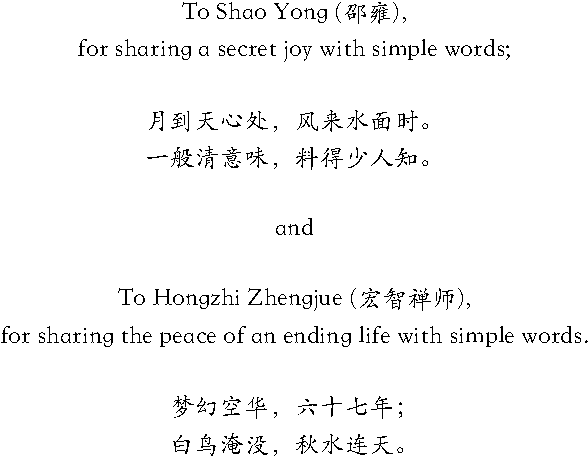
\includegraphics{dedication.pdf}
\end{center}

\setlength{\abovedisplayskip}{-5pt}
\setlength{\abovedisplayshortskip}{-5pt}

{
\setcounter{tocdepth}{1}
\tableofcontents
}
\hypertarget{ID}{%
\chapter*{Prerequisites}\label{ID}}
\addcontentsline{toc}{chapter}{Prerequisites}

This is a \emph{sample} book written in \textbf{Markdown}. You can use anything that Pandoc's Markdown supports, e.g., a math equation \(a^2 + b^2 = c^2\).

The \textbf{bookdown} package can be installed from CRAN\index{CRAN} or Github:

\begin{Shaded}
\begin{Highlighting}[]
\KeywordTok{install.packages}\NormalTok{(}\StringTok{"bookdown"}\NormalTok{)}
\CommentTok{# or the development version}
\CommentTok{# devtools::install_github("rstudio/bookdown")}
\end{Highlighting}
\end{Shaded}

Remember each Rmd file contains one and only one chapter, and a chapter is defined by the first-level heading \texttt{\#}.

To compile this example to PDF, you need XeLaTeX. You are recommended to install TinyTeX (which includes XeLaTeX): \url{https://yihui.org/tinytex/}.

\hypertarget{acerca-del-autor}{%
\chapter*{Acerca del autor}\label{acerca-del-autor}}
\addcontentsline{toc}{chapter}{Acerca del autor}

Los datos consignados son confidenciales

\begin{longtable}[]{@{}rl@{}}
\toprule
Apellidos y Nombres : & MALLQUI BAÑOS, Ricardo Michel\tabularnewline
\midrule
\endhead
Sexo : & Masculino\tabularnewline
Estado civil : & Soltero\tabularnewline
Fecha de nacimiento : & 7 de febrero de 1983\tabularnewline
DNI : & 42131225\tabularnewline
Celular : & 966878340\tabularnewline
Correo : & \href{mailto:ricardomallqui6@gmail.com}{\nolinkurl{ricardomallqui6@gmail.com}}\tabularnewline
Sitio web : & \url{https://github.com/ricardofisma}\tabularnewline
Dirección : & Jr.~Untiveros 452\tabularnewline
\bottomrule
\end{longtable}

\hypertarget{educaciuxf3n-acaduxe9mica}{%
\section*{Educación Académica}\label{educaciuxf3n-acaduxe9mica}}
\addcontentsline{toc}{section}{Educación Académica}

\begin{enumerate}
\def\labelenumi{\arabic{enumi}.}
\item
  \textbf{Licenciado en Ciencias físico matemáticas} -- especialidad \emph{matemática}, Universidad Nacional San Cristóbal de Huamanga.
\item
  \textbf{Bachiller en Ciencias físico matemáticas} -- especialidad \emph{matemática}, Universidad Nacional San Cristóbal de Huamanga.
\item
  \textbf{Maestria -- docencia universitaria} Escuela de posgrado Universidad Nacional San Cristóbal de Huamanga.
\item
  \textbf{Bachiller en Artista Plástico especialidad -- Especialidad escultura} Escuela Superior de Bellas Artes Felipe Guamán Poma de Ayala.
\item
  \textbf{Ingles 5 niveles} en el posgrado Universidad Nacional San Cristóbal de Huamanga.
\item
  Ofimática, Windows, Ms--Word, Ms--Excel, Ms--PowerPoint, Flash, Dreamweaver, Corel Drawn, Photoshop.
\item
  Participación en calidad de \textbf{asistente} en el siglo XX Ciclo de conferencias de matemática, física y estadística, organizado por la escuela de formación profesional de Ciencias Fisco Matemáticas.
\item
  Participación en calidad de \textbf{ponente} en el siglo XX Ciclo de conferencias de matemática, física y estadística, organizado por la escuela de formación profesional de Ciencias Fisco Matemáticas.
\item
  Participación en calidad de \textbf{asistente} en el siglo XXIII Ciclo de conferencias de matemática, física y estadística, organizado por la escuela de formación profesional de Ciencias Fisco Matemáticas.
\item
  Participación en calidad de \textbf{asistente} en el siglo XXIII Ciclo de conferencias de matemática, física y estadística, organizado por la escuela de formación profesional de Ciencias Fisco Matemáticas.
\item
  Participación en calidad de \textbf{asistente} en el I Curso Taller Didáctica De Las Artes Visuales en el Nivel Superior, organizado por la escuela de bellas artes Felipe Guman Poma de Ayala.
\end{enumerate}

\hypertarget{desarrollo-laboral}{%
\section*{Desarrollo Laboral}\label{desarrollo-laboral}}
\addcontentsline{toc}{section}{Desarrollo Laboral}

\begin{enumerate}
\def\labelenumi{\arabic{enumi}.}
\item
  Docencia en matemáticas 1 semestre de experiencia Universidad Nacional San Cristóbal de Huamanga.
\item
  Docencia en matemáticas 1 siclo de experiencia en la CEPRE -- Universidad Nacional San Cristóbal de Huamanga.
\item
  Docencia en matemáticas 2 años de experiencia (IE Mirtha Heri de añaños San Miguel y IE Señor de los Milagros San Miguel).
\item
  Docencia de dibujo -- escultura dos años de experiencia (Escuela superior de bellas arte Felipe Guaman Poma de Ayala)
\item
  Exposición individual de escultura.
\item
  Trabajos encargados de escultura.
\item
  Editor de textos científicos con LaTeX.
\end{enumerate}

En 2018 se empezo a utilizar github (\url{https://github.com/ricardofisma})

\hypertarget{introduction}{%
\chapter*{Introduction}\label{introduction}}
\addcontentsline{toc}{chapter}{Introduction}

You can write citations, too. For example, we are using the \textbf{bookdown} package \citep{R-bookdown} in this sample book, which was built on top of R Markdown and \textbf{knitr} \citep{xie2015}.

\mainmatter

\hypertarget{derivaciuxf3n}{%
\chapter{Derivación}\label{derivaciuxf3n}}

En este capítulo se trata de funciónes\index{funciónes} que cambian de valor al variar el valor de la variable independiente. Al establecer esta relación y medirla presisamente concierne al Cálculo Diferencial. Newton al estudiar dos variables relacionados descubrió estos principios llamados inicialmente \emph{fluxiones}\index{fluxiones} un instrumento matemático hasta hoy significativo en muchas ramas del conocimiento.

Un \emph{incremento} de una variable de un valor númerico a otro, es la \emph{diferencia} que se obtiene de restar el primer valor del segundo. Un incremento de una variable \(x\) se representa por el simbolo \(\Delta x\) leida como ``delta de \(x\)'' o delta veces \(x\)

Evidentemente el incremento\index{incremento} puede ser engativo o positivo de acuerdo a si la variable aumenta o disminuye.

Sea la función

\begin{equation}
y=x^2
\label{eq:r}
\end{equation}
sea \(x\) fijo entonces un incremento \(\Delta x\) implica in incremento en \(y\) de \(\Delta y\) se obtiene

\begin{equation}
y+\Delta y=(x+\Delta x)^2=x^2+2x\Delta x+(\Delta x)^2
\label{eq:rr}
\end{equation}

entonces restando \eqref{eq:r} de \eqref{eq:rr} se obtiene el \emph{incremento} \(\Delta y\) en función de \(x\) y \(\Delta x\)

\begin{equation}
\Delta y=2x\Delta x+(\Delta x)^2
\label{eq:rrr}
\end{equation}

Luego la razón de los incrementos se obtiene al dividir por \(\Delta x\) ambos mienbros de \eqref{eq:rrr} \[\frac{\Delta y}{\Delta x}=2x+\Delta x\] entonces el limite en \(x=4\) es \[\lim_{\Delta x\to 0}\frac{\Delta y}{\Delta x}=2\cdot 4+0=8\]

La \emph{dderivada} de una fucnion de una variable

\hypertarget{methods}{%
\chapter{Methods}\label{methods}}

We describe our methods in this chapter.

\hypertarget{example-one}{%
\chapter{Example one}\label{example-one}}

\hypertarget{example-two}{%
\section{Example two}\label{example-two}}

\hypertarget{example-twowwwww}{%
\section{Example twowwwww}\label{example-twowwwww}}

\hypertarget{example-onewwwww}{%
\chapter{Example onewwwww}\label{example-onewwwww}}

\hypertarget{components}{%
\chapter{Components}\label{components}}

This chapter demonstrates the syntax of common components of a book written in \textbf{bookdown}, including code chunks, figures, tables, citations, math theorems, and equations. The approach is based on Pandoc, so we start with the syntax of Pandoc's\index{Pandoc} flavor of Markdown.

\hypertarget{markdown-syntax}{%
\section{Markdown syntax}\label{markdown-syntax}}

In this section, we give a very brief introduction to Pandoc's Markdown\index{Markdown}. Readers who are familiar with Markdown can skip this section. The comprehensive syntax of Pandoc's Markdown can be found on the Pandoc website \url{http://pandoc.org}.

\hypertarget{appendix-apendice}{%
\appendix \addcontentsline{toc}{chapter}{\appendixname}}


Some \emph{significant} applications are demonstrated in this chapter.

\hypertarget{example-one-1}{%
\chapter{Example one}\label{example-one-1}}

\hypertarget{example-two-1}{%
\section{Example two}\label{example-two-1}}

\hypertarget{example-twowwwww-1}{%
\section{Example twowwwww}\label{example-twowwwww-1}}

\hypertarget{example-onewwwww-1}{%
\chapter{Example onewwwww}\label{example-onewwwww-1}}

\hypertarget{components-1}{%
\chapter{Components}\label{components-1}}

This chapter demonstrates the syntax of common components of a book written in \textbf{bookdown}, including code chunks, figures, tables, citations, math theorems, and equations. The approach is based on Pandoc, so we start with the syntax of Pandoc's\index{Pandoc} flavor of Markdown.

\hypertarget{markdown-syntax-1}{%
\section{Markdown syntax}\label{markdown-syntax-1}}

In this section, we give a very brief introduction to Pandoc's Markdown\index{Markdown}. Readers who are familiar with Markdown can skip this section. The comprehensive syntax of Pandoc's Markdown can be found on the Pandoc website \url{http://pandoc.org}.

\bibliography{book.bib,packages.bib}

\printindex

\end{document}
